\documentclass[11pt,a4paper]{article}

% -----------------------------------------------------------------------------
% Packages
% -----------------------------------------------------------------------------
\usepackage[margin=2.5cm]{geometry}
\usepackage[utf8]{inputenc}
\usepackage[T1]{fontenc}
\usepackage{lmodern}   % scalable Type-1 fonts; required so microtype font-expansion works on a fresh MiKTeX
\usepackage{microtype}
\usepackage{amsmath}
\usepackage{booktabs}
\usepackage{longtable}
\usepackage{array}
\usepackage{float}
\usepackage{graphicx}
\graphicspath{{../presentation/images/schematic_blocks/}{../presentation/images/}}
\usepackage{xcolor}
\usepackage{listings}
\usepackage{hyperref}
\usepackage{enumitem}
\usepackage{tikz}
\usetikzlibrary{arrows.meta, positioning, shapes, fit, calc, automata}

% Allow slightly looser line breaking to avoid overfull boxes in tables/lists.
\emergencystretch=1em

% -----------------------------------------------------------------------------
% Colors and styles
% -----------------------------------------------------------------------------
\definecolor{nodeblue}{RGB}{63, 114, 175}
\definecolor{nodegreen}{RGB}{46, 139, 87}
\definecolor{nodered}{RGB}{192, 57, 43}
\definecolor{nodegray}{RGB}{120, 120, 120}
\definecolor{backgray}{RGB}{245, 245, 245}

\tikzset{
    appnode/.style={
        rectangle,
        rounded corners=4pt,
        draw=nodeblue,
        fill=nodeblue!10,
        line width=1.2pt,
        minimum width=4.2cm,
        minimum height=2.2cm,
        align=center,
        font=\sffamily\small
    },
    io/.style={
        rectangle,
        rounded corners=3pt,
        draw=#1,
        fill=#1!8,
        line width=1pt,
        minimum width=2.8cm,
        minimum height=1cm,
        align=center,
        font=\sffamily\small
    },
    bus/.style={
        ->,
        >=Stealth,
        line width=1pt
    },
    databus/.style={
        <->,
        >=Stealth,
        line width=1pt,
        dashed
    }
}

\lstset{
    basicstyle=\ttfamily\small,
    backgroundcolor=\color{backgray},
    frame=single,
    framerule=0pt,
    breaklines=true,
    columns=flexible,
    keepspaces=true
}

% -----------------------------------------------------------------------------
% Metadata
% -----------------------------------------------------------------------------
\title{
    \textbf{SecurityNode}\\[0.4em]
    \Large Application Note\\
    Controller / Application Node Design
}
\author{Final Project of Electronic Design}
\date{Version~1.1 (schematic-verified) --- \today}

\begin{document}

\maketitle

\begin{abstract}
This application note documents the \textbf{design} of the SecurityNode
controller/application node.  The node is implemented on the
ESP32-C3-WROOM-02-N4 and is responsible for sensor monitoring, alarm control,
vision-module coordination, and host communication.  Because the project is
still at the design stage and no assembled hardware is available, this note
focuses on architectural choices, electrical interfaces, requirements and
traceability, a formal state machine, the UART protocol, and a theoretical
verification plan.  Measured bench data such as oscilloscope waveforms, thermal
tests, and power-consumption plots are intentionally excluded.

\medskip
\noindent\textbf{Status and verification note:} This is a design-stage,
not-yet-fabricated project: no hardware has been built and no firmware has been
written.  The \emph{pin map and electrical facts} in this note (pinout, power
tree, U4/U5 roles, designators) are \textbf{verified against the schematic
netlist}.  All \emph{firmware, communication-protocol, finite-state-machine,
and host-tool content is a PROPOSED design}, not as-built, and is labelled as
such throughout.
\end{abstract}

\begin{center}\small
\begin{tabular}{@{}clp{8.4cm}@{}}
\toprule
\textbf{Rev.} & \textbf{Date} & \textbf{Change} \\
\midrule
1.0 & --- & Initial design-stage application note. \\
1.1 & \today & Pinout, power tree, and U4/U5 roles corrected and verified against the schematic netlist; schematic/PCB figures, component-value rationale, key-components table, and references added. \\
\bottomrule
\end{tabular}
\end{center}

\tableofcontents
\newpage

% -----------------------------------------------------------------------------
\section{Purpose and scope}
% -----------------------------------------------------------------------------

This application note has three objectives:

\begin{enumerate}
    \item Capture the design intent of the SecurityNode application/controller node.
    \item Provide enough detail for a peer review of the firmware architecture,
        electrical interfaces, and communication protocol before hardware is built.
    \item Define the verification activities that can be performed analytically
        or by inspection, given that no physical prototype exists yet.
\end{enumerate}

The note covers:

\begin{itemize}
    \item Design assumptions and constraints.
    \item Design artifacts produced by the project.
    \item Functional requirements and a traceability matrix.
    \item External interfaces and a formal pinout.
    \item Electrical design summary and review notes.
    \item Finite-state machine with a camera-availability flag.
    \item UART protocol interface between the ESP32-C3 and the ESP32-CAM.
    \item Firmware design sketch.
    \item Theoretical verification plan.
\end{itemize}

The following topics are \textbf{out of scope} until hardware is fabricated:
measured waveforms, oscilloscope captures, thermal performance, real power
consumption, and PCB bring-up results.

% -----------------------------------------------------------------------------
\section{Design assumptions}
% -----------------------------------------------------------------------------

The design described in this note relies on the assumptions listed in
Table~\ref{tab:assumptions}.

\begin{table}[H]
    \centering
    \caption{Design assumptions.}
    \label{tab:assumptions}
    \begin{tabular}{@{}clp{8cm}@{}}
        \toprule
        \textbf{ID} & \textbf{Area} & \textbf{Assumption} \\
        \midrule
        A1 & Controller & The application node runs on an ESP32-C3-WROOM-02-N4. \\
        A2 & Vision & The ESP32-CAM is connected through UART1 on IO0=RX / IO1=TX (auto-isolated by U5, a CAM-presence-gated series switch) at 115200~baud. \\
        A3 & Sensors & The door contact and PIR (the PIR is 5~V-powered, its signal reaching the C3 through a clamp/divider network) reach the C3 as logic-level signals; polarity is configurable in firmware. \\
        A4 & Power & The board is powered from a 5~V USB source through a PTC fuse (F1); a 5~V rail then feeds, in parallel, the 3.3~V LDO (U1) for the C3+U5 logic and the CAM power gate (U4). \\
        A5 & Outputs & The buzzer is driven by a low-side N-channel MOSFET (Q1, DN2302S); the alarm LED (D5) has a series current-limiting resistor (R15, 330~$\Omega$). \\
        A6 & Host & The C3 is programmed and debugged over its \textbf{native USB} (USB-Serial/JTAG, IO18/IO19); a separate UART0 debug header (J1, GPIO20/21) is also provided. No USB-UART bridge chip is present. \\
        A7 & Algorithm & The ESP32-CAM returns one of the result codes defined in the CAM protocol; the C3 does not run vision inference. The on-device vision approach is a \emph{deliberately open design decision} (see \S\ref{sec:vision}). \\
        A8 & Backup & No battery backup is provided; the system operates from USB power only. \\
        \bottomrule
    \end{tabular}
\end{table}

% -----------------------------------------------------------------------------
\section{Design artifacts}
% -----------------------------------------------------------------------------

The following artifacts are part of the SecurityNode design baseline and are
referenced throughout this note:

\begin{itemize}
    \item \texttt{docs/system/system\_overview.md} --- System description and block diagram.
    \item \texttt{docs/firmware/firmware\_architecture.md} --- Firmware structure and build options.
    \item \texttt{docs/firmware/cam\_protocol.md} --- Binary UART protocol specification.
    \item \texttt{docs/hardware/} --- Hardware interface notes and design rationale.
    \item \texttt{hardware/altium/} --- \emph{Planned} Altium schematic and PCB source files (directory is currently a placeholder; the schematic netlist and BOM are the present source of truth).
    \item \texttt{firmware/}, \texttt{software/host/} --- \emph{Planned} firmware and host-tool source (directories are currently placeholders; no code written yet).
    \item \texttt{assets/Schematic Blocks/} --- Schematic-block previews.
    \item \texttt{assets/pcb.pdf} --- PCB fabrication preview.
    \item This document --- Application Note for the controller node.
\end{itemize}

% -----------------------------------------------------------------------------
\section{Requirements}
% -----------------------------------------------------------------------------

\begin{table}[H]
    \centering
    \caption{Controller/Application Node functional requirements.}
    \label{tab:requirements}
    \begin{tabular}{>{\raggedright\arraybackslash}p{0.7cm} >{\raggedright\arraybackslash}p{3.6cm} >{\raggedright\arraybackslash}p{4.5cm} c >{\raggedright\arraybackslash}p{2.6cm}}
        \toprule
        \textbf{ID} & \textbf{Requirement} & \textbf{Rationale} & \textbf{Priority} & \textbf{Verification} \\
        \midrule
        R1 & Monitor door contact continuously. & Detect unauthorized entry. & High & Inspection / Analysis \\
        R2 & Monitor PIR motion continuously. & Detect movement inside the protected area. & High & Inspection / Analysis \\
        R3 & Request visual verification from the ESP32-CAM on a sensor event. & Gate the alarm on visual evidence: catch masked / covered-face intruders while suppressing benign triggers. & High & Protocol review \\
        R4 & Activate the local alarm when a suspicious condition is detected. & Deter intruders and alert occupants. & High & State-machine review \\
        R5 & Operate as a basic alarm when the vision module is unavailable. & Maintain security even if the CAM fails. & High & State-machine review \\
        R6 & Provide a debug/configuration channel: native USB (USB-Serial/JTAG) plus a UART0 header (J1). & Allow setup, diagnostics, and logging. & Medium & Interface test \\
        R7 & Recover from transient UART errors through retry and timeout. & Improve communication robustness. & Medium & Protocol review \\
        R8 & Operate from a 5~V USB supply within standard current limits. & Simplify deployment and avoid overload. & Medium & Power budget analysis \\
        \bottomrule
    \end{tabular}
\end{table}

% -----------------------------------------------------------------------------
\section{Traceability matrix}
% -----------------------------------------------------------------------------

Table~\ref{tab:traceability} maps each requirement to the sections of this note
that address it and the planned verification method.

\begin{table}[H]
    \centering
    \caption{Requirements traceability matrix.}
    \label{tab:traceability}
    \begin{tabular}{>{\raggedright\arraybackslash}p{1.0cm} >{\raggedright\arraybackslash}p{4.4cm} >{\raggedright\arraybackslash}p{5.4cm}}
        \toprule
        \textbf{Req.} & \textbf{Addressed in} & \textbf{Verification activity} \\
        \midrule
        R1 & \S\ref{sec:pinout}, \S\ref{sec:statemachine}, \S\ref{sec:sketch} & GPIO input review; state coverage analysis. \\
        R2 & \S\ref{sec:pinout}, \S\ref{sec:statemachine}, \S\ref{sec:sketch} & GPIO input review; state coverage analysis. \\
        R3 & \S\ref{sec:uart}, \S\ref{sec:statemachine} & Protocol inspection; state-transition review. \\
        R4 & \S\ref{sec:statemachine}, \S\ref{sec:electrical} & Alarm-path review; output-drive analysis. \\
        R5 & \S\ref{sec:statemachine} (cam\_available flag) & State-machine review; CAM-failure scenario. \\
        R6 & \S\ref{sec:pinout}, \S\ref{sec:uart} & Native-USB and UART0-header interface review. \\
        R7 & \S\ref{sec:uart} (timeout/retry rules) & Protocol robustness analysis. \\
        R8 & \S\ref{sec:electrical} & Analytical power budget. \\
        \bottomrule
    \end{tabular}
\end{table}

% -----------------------------------------------------------------------------
\section{External interfaces}
% -----------------------------------------------------------------------------
\label{sec:interfaces}

Figure~\ref{fig:appnode-block} shows the controller node and its surrounding
interfaces.

\begin{figure}[H]
    \centering
    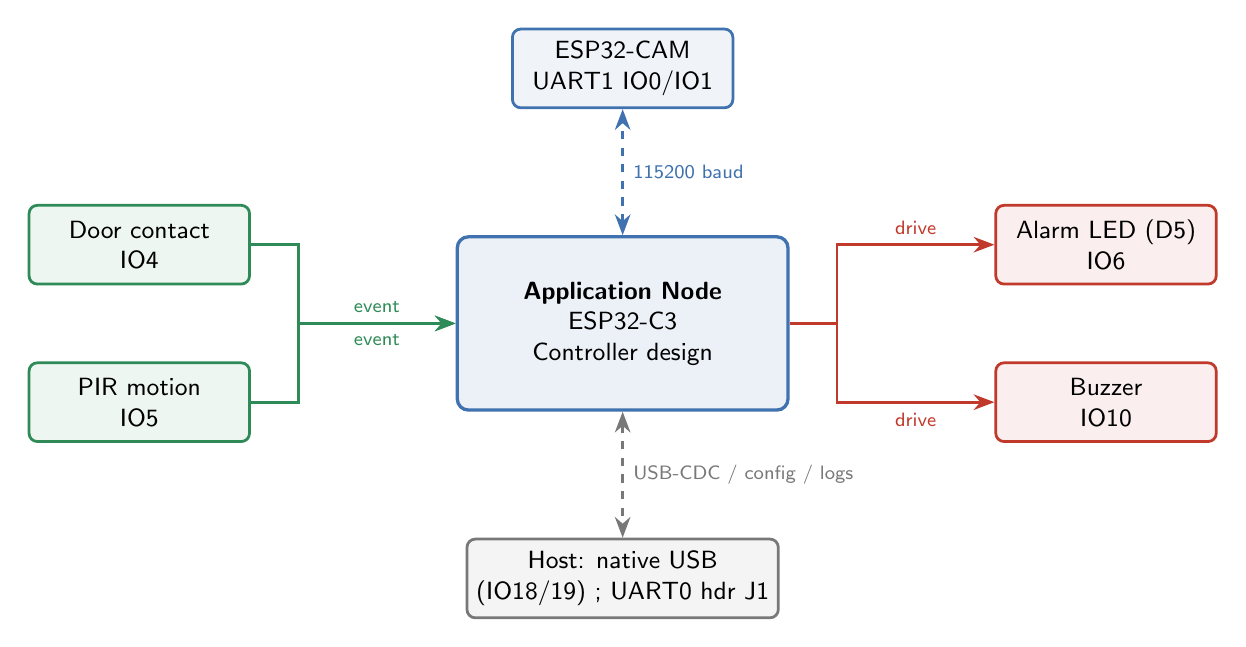
\begin{tikzpicture}[
        node distance=1.4cm and 2.0cm,
        >=Stealth
    ]
        \node[appnode] (app) {\textbf{Application Node}\\ESP32-C3\\Controller design};

        \node[io=nodegreen, left=2.6cm of app, yshift=1.0cm] (door) {Door contact\\IO4};
        \node[io=nodegreen, left=2.6cm of app, yshift=-1.0cm] (pir) {PIR motion\\IO5};

        \node[io=nodered, right=2.6cm of app, yshift=1.0cm] (led) {Alarm LED (D5)\\IO6};
        \node[io=nodered, right=2.6cm of app, yshift=-1.0cm] (buzz) {Buzzer\\IO10};

        \node[io=nodeblue, above=1.6cm of app] (cam) {ESP32-CAM\\UART1 IO0/IO1};

        \node[io=nodegray, below=1.6cm of app] (host) {Host: native USB\\(IO18/19) ; UART0 hdr J1};

        \draw[bus, nodegreen] (door.east) -- ++(0.6,0) |- node[above, pos=0.75, font=\scriptsize\sffamily]{event} (app.west);
        \draw[bus, nodegreen] (pir.east)  -- ++(0.6,0) |- node[below, pos=0.75, font=\scriptsize\sffamily]{event} (app.west);

        \draw[bus, nodered] (app.east) -- ++(0.6,0) |- node[above, pos=0.75, font=\scriptsize\sffamily]{drive} (led.west);
        \draw[bus, nodered] (app.east) -- ++(0.6,0) |- node[below, pos=0.75, font=\scriptsize\sffamily]{drive} (buzz.west);

        \draw[databus, nodeblue] (app.north) -- node[right, font=\scriptsize\sffamily]{115200 baud} (cam.south);

        \draw[databus, nodegray] (app.south) -- node[right, font=\scriptsize\sffamily]{USB-CDC / config / logs} (host.north);
    \end{tikzpicture}
    \caption{Application Node block diagram and external interfaces.}
    \label{fig:appnode-block}
\end{figure}

% -----------------------------------------------------------------------------
\subsection{Pinout}
\label{sec:pinout}
% -----------------------------------------------------------------------------

Table~\ref{tab:pinout} lists the controller pins used by the application node.

\begin{table}[H]
    \centering
    \caption{Application Node pin assignment.}
    \label{tab:pinout}
    \begin{tabular}{>{\raggedright\arraybackslash}p{2.7cm} c c >{\raggedright\arraybackslash}p{2.2cm} >{\raggedright\arraybackslash}p{5.2cm}}
        \toprule
        \textbf{Signal} & \textbf{Pin} & \textbf{Dir.} & \textbf{Function} & \textbf{Electrical notes} \\
        \midrule
        DOOR\_IN & IO4 & Input & Door contact state & Logic-level input; clamp/RC debounce network on board. \\
        PIR\_IN & IO5 & Input & PIR motion detect & PIR powered from 5~V; signal reaches IO5 via clamp/divider; edge or polled. \\
        ALARM\_LED & IO6 & Output & Alarm LED drive & Drives D5 via R15 (330~$\Omega$) series resistor. \\
        BUZZER\_DRV & IO10 & Output & Buzzer MOSFET gate & Drives Q1 (DN2302S) low-side switch via R12; 5~V buzzer load (LS1). \\
        CAM\_TX & IO1 & Output & UART1 TX to ESP32-CAM & 3.3~V, 115200~baud, via R21 + U5; no flow control. \\
        CAM\_RX & IO0 & Input & UART1 RX from ESP32-CAM & 3.3~V, 115200~baud, via R20 + U5; no flow control. \\
        USB\_TX & IO21 & Output & UART0 TX (debug header) & Wired direct to J1 (pin~2); not through U5. \\
        USB\_RX & IO20 & Input & UART0 RX (debug header) & Wired direct to J1 (pin~3); not through U5. \\
        USB\_D & IO18/19 & I/O & Native USB (D$-$/D$+$) & USB-Serial/JTAG to J2 via R3/R4 (22~$\Omega$) + U2 ESD; programming/CDC. \\
        3V3 & --- & Power & Logic supply rail & AP2112K-3.3 LDO (U1) output; feeds C3 + U5 only. \\
        VBUS & --- & Power & 5~V USB input & Over-current protected by PTC fuse F1; TPS2553 (U4) gates CAM\_5V only. \\
        GND & --- & Power & Common ground & Single-point/star grounding per PCB review. \\
        \bottomrule
    \end{tabular}
\end{table}

% -----------------------------------------------------------------------------
\subsection{UART interface parameters}
% -----------------------------------------------------------------------------

\begin{table}[H]
    \centering
    \caption{UART parameters for the ESP32-CAM link.}
    \begin{tabular}{@{}ll@{}}
        \toprule
        \textbf{Parameter} & \textbf{Value} \\
        \midrule
        Controller port & UART1 (IO0=RX / IO1=TX, via U5 isolation switch) \\
        Baud rate & 115200 \\
        Data bits & 8 \\
        Parity & None \\
        Stop bits & 1 \\
        Flow control & None \\
        Frame format & Binary header/length/ID/payload/checksum \\
        \bottomrule
    \end{tabular}
\end{table}

% -----------------------------------------------------------------------------
\subsection{Vision approach (open design decision)}
\label{sec:vision}
% -----------------------------------------------------------------------------

\textbf{This is a deliberately open, design-stage decision.}  The application
node treats the ESP32-CAM as a black box that returns a face-coverage result
code over UART (see the protocol in \S\ref{sec:uart}), but \emph{how} that
result is computed is not yet settled.  A key constraint is that a full
object-detection model (e.g.\ YOLO) does \textbf{not} fit on the ESP32-CAM: the
OV2640-based module is heavily constrained in RAM, flash, and compute.  Three
candidate approaches are under evaluation, each with different trade-offs:

\begin{description}[leftmargin=1.4cm, style=nextline]
    \item[(a) Tiny on-device classifier.] A small quantized classifier
        (ESP-DL or TFLite-Micro) running on the ESP32-CAM, performing a
        coarse \emph{face-present} / \emph{face-covered} judgement on small,
        downscaled frames.  \textit{Trade-off:} fits entirely on-device and
        keeps the architecture single-tier, but offers only modest accuracy and
        limited robustness to pose, lighting, and occlusion variety.
    \item[(b) Off-device inference (two-tier).] The CAM captures a frame and
        streams it over Wi-Fi to a host or edge device running a full model
        (e.g.\ YOLO or a stronger classifier), which returns the verdict.
        \textit{Trade-off:} full accuracy and model flexibility, but requires an
        always-available host and changes the system from one self-contained
        board into a \textbf{two-tier} architecture (latency, networking, and
        availability dependencies).
    \item[(c) Built-in face detection as a coverage proxy.] Use only ESP-DL's
        built-in face-detection primitive and treat ``no detectable face'' as a
        proxy for a covered face.  \textit{Trade-off:} simplest to implement and
        cheapest on-device, but the weakest semantically --- it cannot reliably
        distinguish a \emph{covered face} from \emph{no person present}, which
        risks both false alarms and missed detections.
\end{description}

The choice among (a), (b), and (c) is intentionally left open at this stage; it
should be resolved with an explicit memory/latency budget before firmware is
written.  Assumption~A7 references this open decision rather than asserting any
particular on-device method as settled.

% -----------------------------------------------------------------------------
\section{Electrical design summary}
\label{sec:electrical}
% -----------------------------------------------------------------------------

\subsection{Key components}

Table~\ref{tab:bom} lists the principal devices and their roles; the full
passive network and exact part numbers are in the schematic and the project BOM
(\texttt{assets/SecurityNode.BomDoc}).

\begin{table}[H]
    \centering
    \caption{Key components (designator $\rightarrow$ part $\rightarrow$ role).}
    \label{tab:bom}
    \begin{tabular}{@{}l >{\raggedright\arraybackslash}p{4.4cm} >{\raggedright\arraybackslash}p{6.2cm}@{}}
        \toprule
        \textbf{Ref.} & \textbf{Part} & \textbf{Role} \\
        \midrule
        U1 & AP2112K-3.3TRG1 & 3.3~V / 600~mA LDO (logic rail). \\
        U2 & USBLC6-2P6 & USB D+/D$-$ ESD protection. \\
        U3 & ESP32-C3-WROOM-02-N4 & Controller / application node. \\
        U4 & TPS2553DBVR & ESP32-CAM power gate (adjustable current limit). \\
        U5 & SN74LVC2G66DCTR & CAM-presence-gated UART1 isolation switch. \\
        Q1 & DN2302S & N-MOSFET low-side buzzer driver. \\
        LS1 & KPEG242-5V & Buzzer (5~V). \\
        D5 & XL-2012SURC & Red 0805 alarm LED. \\
        D1 & SMF5.0CA & VBUS input TVS clamp. \\
        F1 & Littelfuse 1206L075/16V & PTC resettable fuse (input over-current). \\
        FB1 & HCB1608KF-600T20 & 60~$\Omega$ ferrite bead (input EMI filter). \\
        J2 & KH-MINI-SMT-5P (Mini-USB~B) & 5~V input + native-USB data. \\
        J3 & ESP32-CAM (AI-Thinker) & Vision-module mezzanine connector. \\
        J1 / J7 & Pin headers & ESP32-C3 / ESP32-CAM programming \& debug. \\
        \bottomrule
    \end{tabular}
\end{table}

\subsection{Power architecture}

The board receives 5~V (VBUS) from a Mini-USB connector (J2).  The input chain
is: VBUS $\rightarrow$ \textbf{F1} (PTC resettable fuse; whole-board over-current
protection) $\rightarrow$ \textbf{D1} (input TVS clamp) with \textbf{C1} bulk
capacitor $\rightarrow$ \textbf{FB1} (ferrite bead) $\rightarrow$ the
\textbf{5~V rail}.  The 5~V rail then feeds, \emph{in parallel}, the
\textbf{U1} (AP2112K-3.3) LDO and the \textbf{U4} (TPS2553) CAM power gate, as
well as the buzzer (LS1) and the PIR supply.

The \textbf{3.3~V rail} (U1 output) feeds \textbf{only the ESP32-C3 (U3) and the
U5 switch} plus logic pull-ups.  The buzzer and PIR run directly on the
\textbf{5~V rail}.  The ESP32-CAM runs on \texttt{CAM\_5V} --- the gated output
of U4 --- together with its own internal \texttt{CAM\_3V3} regulator output; the
on-board LDO does not power the CAM.  ESD protection on the USB data lines is
provided by U2 (USBLC6-2P6) with series 22~$\Omega$ resistors; input-line TVS
clamping uses SMF5.0CA devices.  U4 does \emph{not} distribute power board-wide
--- whole-board USB over-current protection is the job of F1.

\subsection{Camera power gate (U4) and UART isolation switch (U5)}

\textbf{U4 (TPS2553) --- ESP32-CAM power gate only.}  U4 is an adjustable
current-limited power switch dedicated to the camera: input is the 5~V rail,
output is \texttt{CAM\_5V}.  It is enabled by \texttt{CAM\_EN} from the C3
(IO7, through R9), its current limit is set by R13 (21.5~k$\Omega$), and its
\texttt{FAULT} output feeds back to the C3 on IO3.  An R11 (100~k$\Omega$)
pulldown holds the gate \textbf{OFF by default} during C3 boot, so the camera is
powered only when the controller explicitly enables it.  U4 does not feed the
5~V rail, the LDO, or the buzzer.

\textbf{U5 (SN74LVC2G66) --- automatic CAM-presence-gated UART isolation
switch.}  U5 is a two-channel analog switch placed in series on the
C3$\leftrightarrow$CAM UART1 link (both directions of \texttt{CAM\_TXD}/%
\texttt{CAM\_RXD}).  Its control pins are hard-tied to the camera's own
\texttt{CAM\_3V3} output, so the link \emph{auto-connects} only when a powered
CAM module is seated and \emph{auto-disconnects} when the CAM is absent or off.
U5 is \textbf{not} a USB-to-UART programming multiplexer and is not
host/GPIO-selectable.

\subsection{Analytical power budget}

Because no hardware has been built, the budget in Table~\ref{tab:power} is an
analytical estimate used to size the input supply, the F1 PTC fuse, and the U4
current limit, and to determine which USB source the deployment requires.  The
3.3~V loads are referred to the 5~V input on the assumption that the AP2112K is
a linear LDO (input current $\approx$ output current), so the per-rail currents
can be summed into a single 5~V-input figure.

\begin{table}[H]
    \centering
    \caption{Estimated application-node power budget.}
    \label{tab:power}
    \begin{tabular}{@{}>{\raggedright\arraybackslash}p{6.4cm}ccc@{}}
        \toprule
        \textbf{Load} & \textbf{Voltage (V)} & \textbf{Current (mA)} & \textbf{Power (mW)} \\
        \midrule
        ESP32-C3 active & 3.3 & 80 & 264 \\
        ESP32-CAM peak (Wi-Fi + camera on, on \texttt{CAM\_5V}) & 5.0 & 500 & 2500 \\
        Alarm LED (D5), $\approx(3.3-2.0)/330$ & 3.3 & 4 & 13 \\
        Buzzer (5~V rail through MOSFET; alarm state only) & 5.0 & 40 & 200 \\
        Door contact / PIR leakage & 3.3 & 2 & 7 \\
        \midrule
        \textbf{Total (peak: CAM + alarm active)} & --- & \textbf{626} & \textbf{2984} \\
        \bottomrule
    \end{tabular}
\end{table}

The dominant load is the ESP32-CAM during a Wi-Fi + capture burst, drawn on the
gated \texttt{CAM\_5V} branch.  With the camera enabled, the estimated peak
($\approx$~626~mA) exceeds a basic 500~mA USB port, so the deployment supply
must provide headroom: a 5~V/1~A (or better) source is recommended, and the F1
PTC fuse (750~mA hold / 1.5~A trip) and the U4 current limit (set by R13) must be
coordinated with this peak (see \S\ref{sec:values}).  Because the camera is
power-gated by U4 and held OFF by default (R11), the \emph{monitoring quiescent}
draw with the CAM disabled (C3 + alarm LED + sensors, $\approx 80+4+2$~mA) is
only about 90~mA --- well within a 500~mA USB port; sounding the buzzer in the
ALARM state adds roughly 40~mA.  These magnitudes are analytical estimates to be
confirmed by bench measurement once hardware exists.

\subsection{Output drive}

The buzzer is switched by Q1, a DN2302S N-channel MOSFET.  The ESP32-C3 GPIO
(IO10) drives the Q1 gate through an R12 (100~$\Omega$) series resistor, with an
R14 (10~k$\Omega$) gate pulldown to keep the buzzer off during reset/boot; the
gate threshold and on-resistance must be checked against the buzzer current in
the final schematic review.  The alarm LED (D5) is driven from IO6 through an
R15 (330~$\Omega$) series resistor sized for the desired LED current and forward
voltage.

\subsection{Component value rationale}
\label{sec:values}

The load-bearing component values are justified below; values inferred from the
net topology rather than an explicit annotation are flagged for confirmation
against the Altium source.

\begin{itemize}
    \item \textbf{Alarm-LED resistor R15 (330~$\Omega$).}  With a red LED forward
        voltage $V_f\approx2.0$~V driven from the 3.3~V output IO6,
        \[ I_{LED}=\frac{3.3-V_f}{R_{15}}=\frac{3.3-2.0}{330}\approx 3.9~\text{mA}, \]
        a safe, clearly visible indicator current within the GPIO drive
        capability (the $\approx4$~mA used in the power budget).
    \item \textbf{Buzzer MOSFET Q1 (DN2302S) gate drive.}  The DN2302S is a
        logic-level N-channel device ($V_{GS(th)}\approx1.0$--$1.5$~V), so the
        3.3~V drive from IO10 fully enhances it; at the $\approx40$~mA buzzer
        current its $R_{DS(on)}$ drop is negligible.  R12 (100~$\Omega$) limits
        gate inrush and R14 (10~k$\Omega$) holds the gate low (buzzer off) while
        IO10 is high-impedance during reset/boot.
    \item \textbf{CAM power-gate limit, U4 (TPS2553) with R13 (21.5~k$\Omega$).}
        The TPS2553 programmable limit follows the datasheet $I_{OS}$--$R_{ILIM}$
        relationship over a 0.075--1.7~A range; R13 sits near the low end of the
        resistor range, programming a limit in the upper part of that span (order
        of $\approx1.5$~A --- the exact threshold to be read from the TPS2553
        datasheet equation for $R_{ILIM}=21.5$~k$\Omega$).  This is above the
        camera's $\approx500$~mA peak, so normal operation is not throttled,
        while it still caps a CAM fault.  Because this limit is close to the F1
        PTC trip current ($\approx1.5$~A), the two must be coordinated so the gate
        limits before the board fuse trips --- a point to confirm in review.
    \item \textbf{Sensor input conditioning.}  The door (J4) and PIR (J5) inputs
        use an RC + clamp network to bound the GPIO voltage and pre-filter
        contact bounce / EMI, complemented by an $\approx50$~ms firmware debounce
        (\S\ref{sec:statemachine}).  The PIR is 5~V-powered, so its output is made
        3.3~V-compatible to IO5 by the on-board clamp/divider; the exact RC
        constant and divider ratio are to be confirmed against the schematic.
\end{itemize}

\subsection{Schematic preview}

The schematic is partitioned into the functional blocks in
Figures~\ref{fig:blk-power}--\ref{fig:blk-io}: power input and regulation, the
ESP32-C3 controller, the ESP32-CAM interface, the sensor inputs, and the alarm
outputs.  (The UART isolation switch U5 is detailed in the previous subsection.)

\begin{figure}[H]
    \centering
    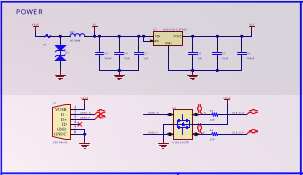
\includegraphics[width=0.82\linewidth]{power}
    \caption{Power input, protection, and regulation: USB $\rightarrow$ F1 (PTC)
    $\rightarrow$ D1 (TVS) $\rightarrow$ FB1 $\rightarrow$ 5\,V rail $\rightarrow$
    U1 (AP2112K) 3.3\,V LDO, with U4 (TPS2553) gating \texttt{CAM\_5V}.}
    \label{fig:blk-power}
\end{figure}

\begin{figure}[H]
    \centering
    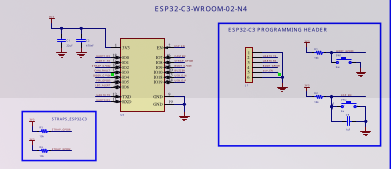
\includegraphics[width=0.48\linewidth]{esp32c3}\hfill
    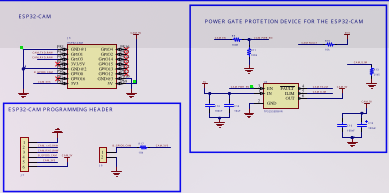
\includegraphics[width=0.48\linewidth]{esp32cam}
    \caption{ESP32-C3 controller block (left) and ESP32-CAM interface block,
    including the U5 UART-isolation switch (right).}
    \label{fig:blk-mcu}
\end{figure}

\begin{figure}[H]
    \centering
    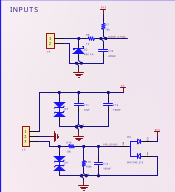
\includegraphics[width=0.48\linewidth]{inputs}\hfill
    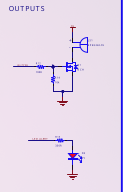
\includegraphics[width=0.48\linewidth]{outputs}
    \caption{Sensor input conditioning (door / PIR, left) and alarm output
    drivers (LED and MOSFET-driven buzzer, right).}
    \label{fig:blk-io}
\end{figure}

\subsection{PCB design review notes}

\begin{figure}[H]
    \centering
    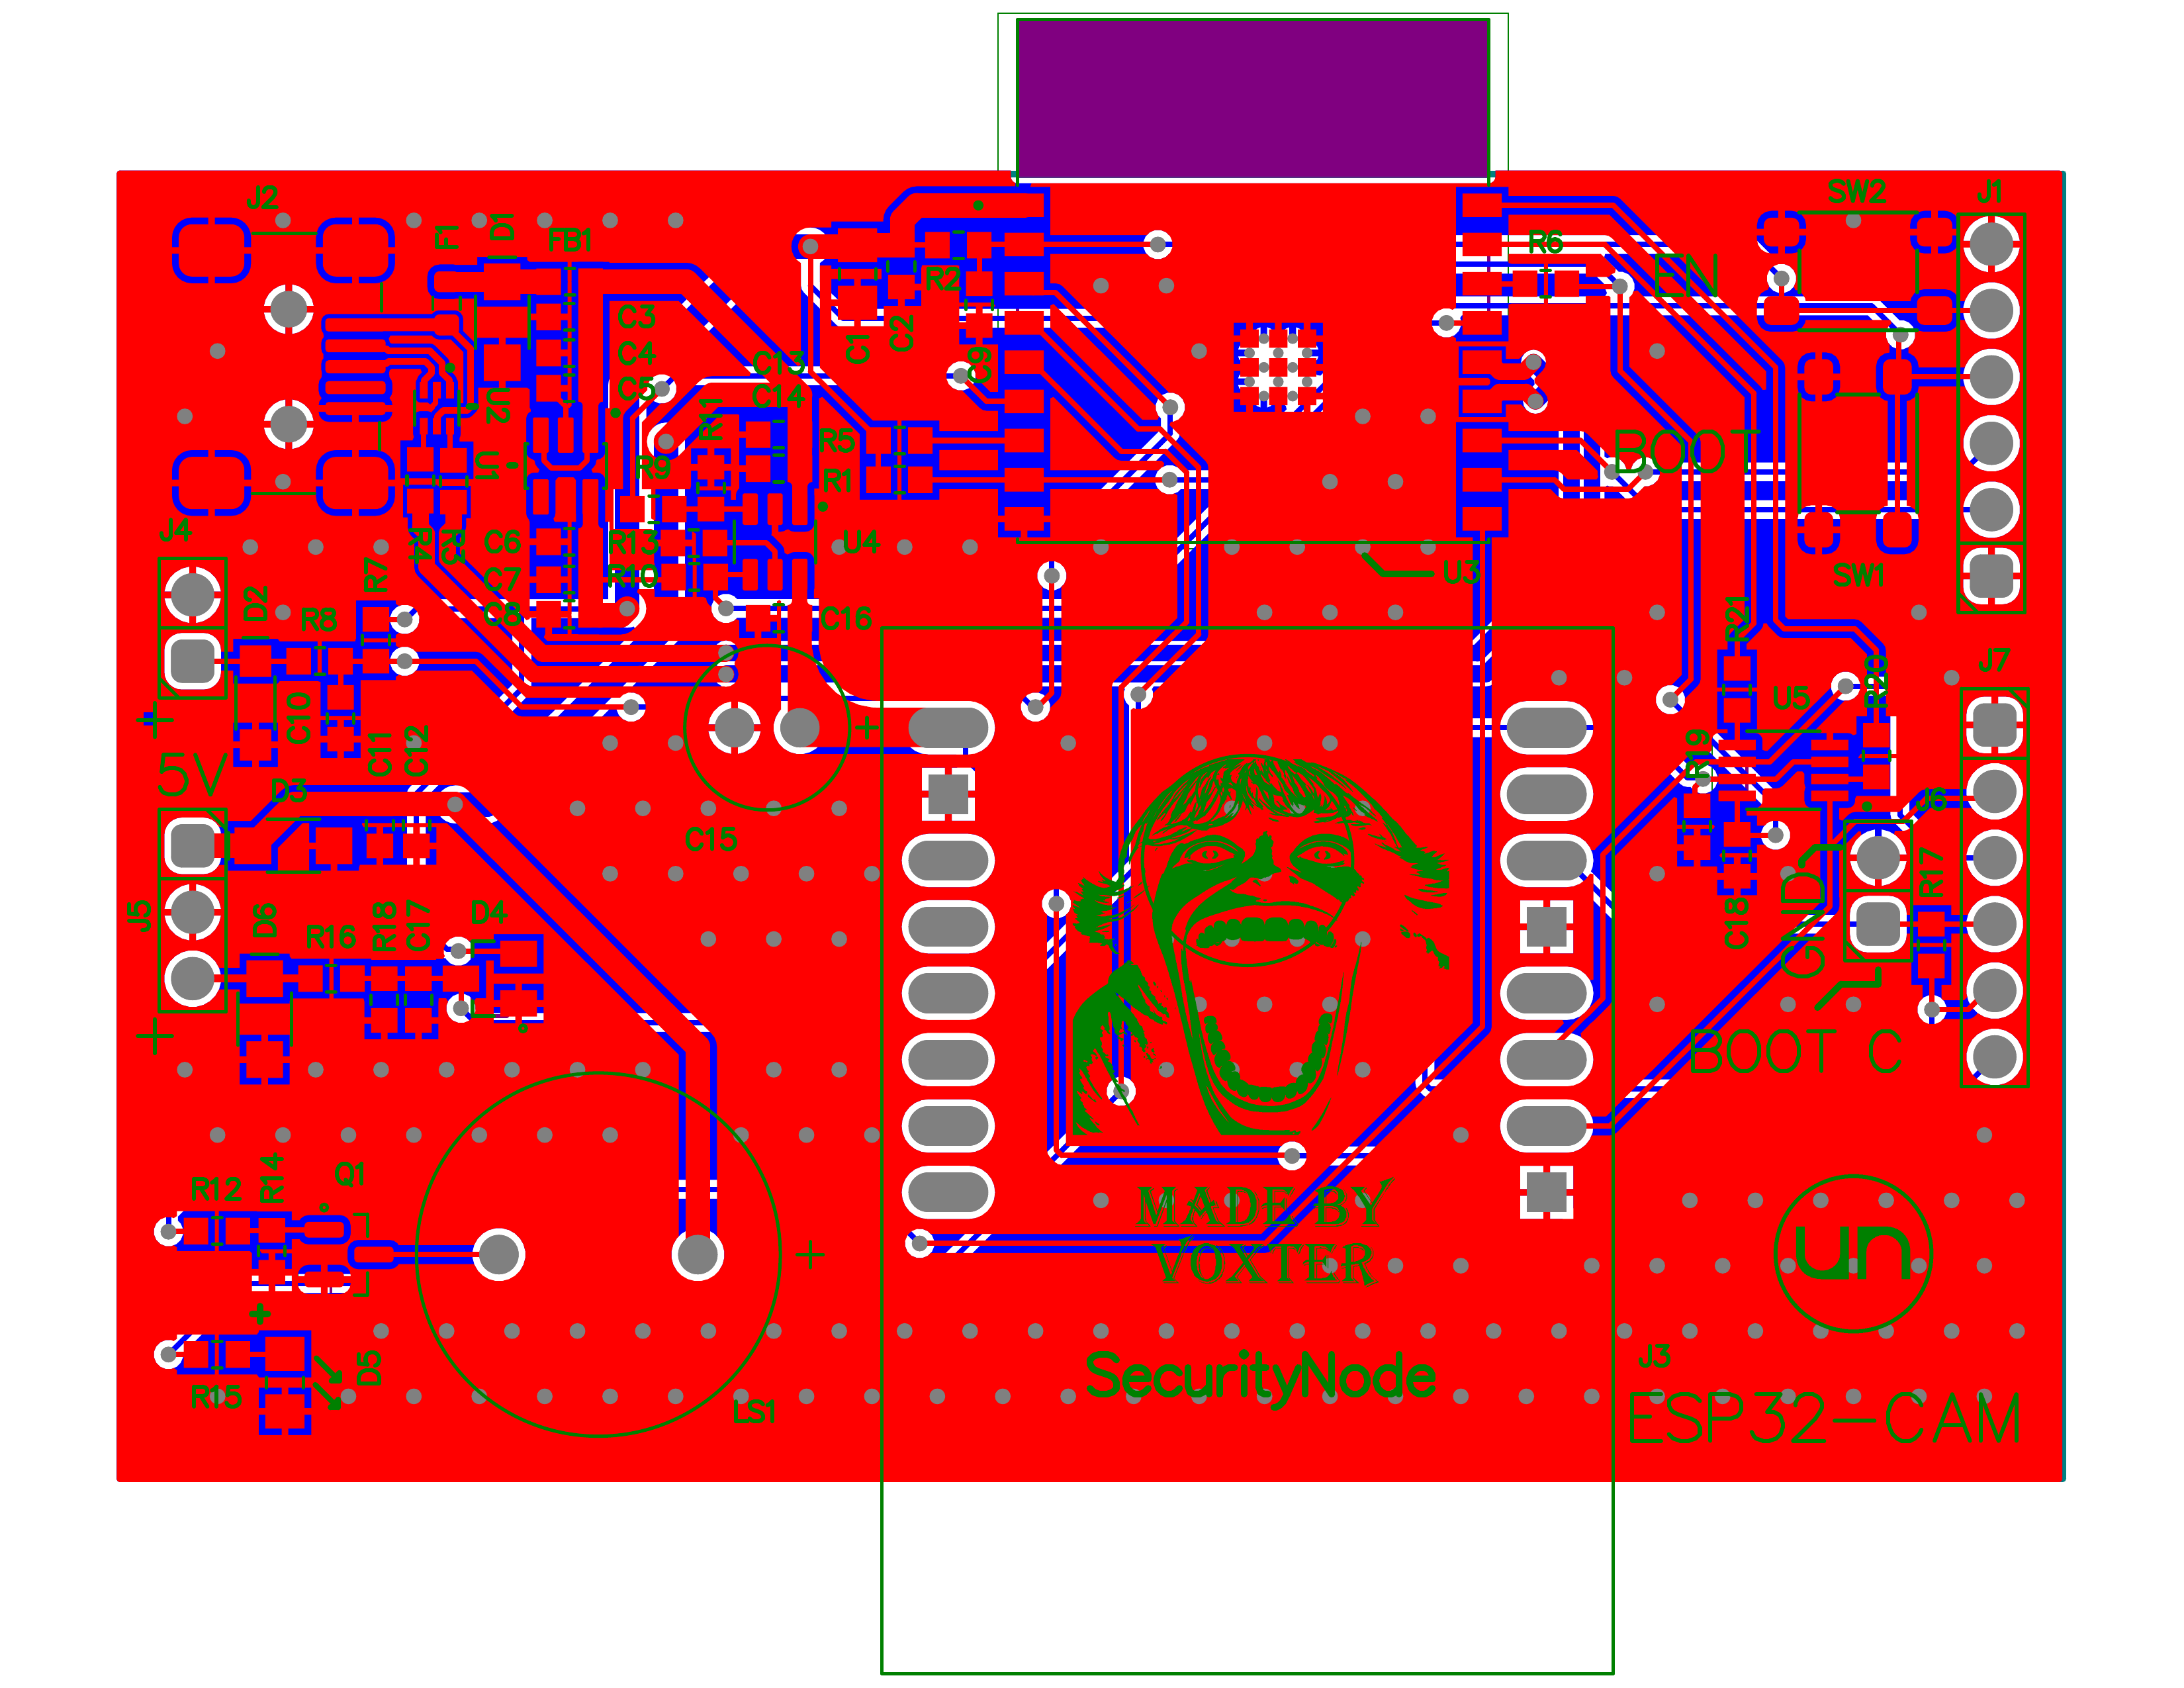
\includegraphics[width=0.55\linewidth]{pcb_2d}
    \caption{PCB layout preview (2-D top view).  3-D top/bottom renders are
    available under \texttt{assets/}.}
    \label{fig:pcb}
\end{figure}

Before fabrication, the PCB layout should be reviewed against the following
checklist:

\begin{itemize}
    \item Keep the UART1 traces between the ESP32-C3 and ESP32-CAM short and matched.
    \item Place decoupling capacitors close to each IC power pin.
    \item Provide a solid ground plane under the microcontroller and camera module.
    \item Route the buzzer load away from sensitive sensor traces to reduce switching noise.
    \item Confirm the native-USB data path (J2 $\rightarrow$ U2 USBLC6 ESD $\rightarrow$ R3/R4 22~$\Omega$ series $\rightarrow$ IO18/IO19) has the required ESD protection and matched series resistors.
    \item Verify the CAM power-gate enable/fault path: \texttt{CAM\_EN} (IO7 $\rightarrow$ R9 $\rightarrow$ U4 EN), the default-OFF pulldown (R11), the ILIM resistor (R13), and \texttt{FAULT} back to IO3.
    \item Verify the U5 series-isolation switch on the UART1 link is gated by \texttt{CAM\_3V3} (auto presence-gating), not routed as a programmable mux.
\end{itemize}

% -----------------------------------------------------------------------------
\section{State machine}
\label{sec:statemachine}
% -----------------------------------------------------------------------------

The application behavior is modelled as a finite-state machine.  A new state,
\textbf{INCONCLUSIVE}, replaces the previous ``CLEAR'' state: rather than
asserting that a visible (or absent) face is \emph{safe}, the node only records
that it found \emph{no positive evidence of a covered face} --- a covered face is
the sole condition that escalates to ALARM through the vision path.  This is a
deliberate semantic distinction; to make it behavioural as well, repeated
INCONCLUSIVE results within a short window may be counted toward escalation (a
configurable threshold), so a stream of unreadable captures does not silently
re-arm forever.  The \textbf{ARMED} state maintains a \texttt{cam\_available}
flag, updated by periodic status queries, that determines whether the node can
enter the vision-verification path or must fall back to basic-alarm behavior.

\subsection{State definitions}

\begin{itemize}
    \item \textbf{INIT} --- System startup, self-test, GPIO/UART initialization, and initial CAM presence check.
    \item \textbf{ARMED} --- Normal monitoring mode.  LED slow-blinks, sensors are active, and the node periodically queries the CAM status to set \texttt{cam\_available}.
    \item \textbf{TRIGGERED} --- A sensor event has been detected.  The LED fast-blinks.  If \texttt{cam\_available} is true, the node proceeds to visual verification; otherwise it enters the ALARM state as a basic alarm.
    \item \textbf{VISION\_REQUEST} --- The node sends CMD\_CAPTURE to the ESP32-CAM and waits for an ACK.
    \item \textbf{VISION\_CHECK} --- The node waits for the analysis result while maintaining the fast-blink indication.  A 5~s timeout is enforced.
    \item \textbf{INCONCLUSIVE} --- The CAM reports a visible face, no face, or another non-threat condition.  The event is logged and the node returns to ARMED without sounding the alarm.
    \item \textbf{ALARM} --- A suspicious condition, communication failure, or CAM-unavailable condition has occurred.  The LED is solid and the buzzer is ON until the node is disarmed or the alarm timeout expires.
\end{itemize}

\subsection{State-transition diagram}

Figure~\ref{fig:appnode-fsm} shows the updated state machine.

\begin{figure}[H]
    \centering
    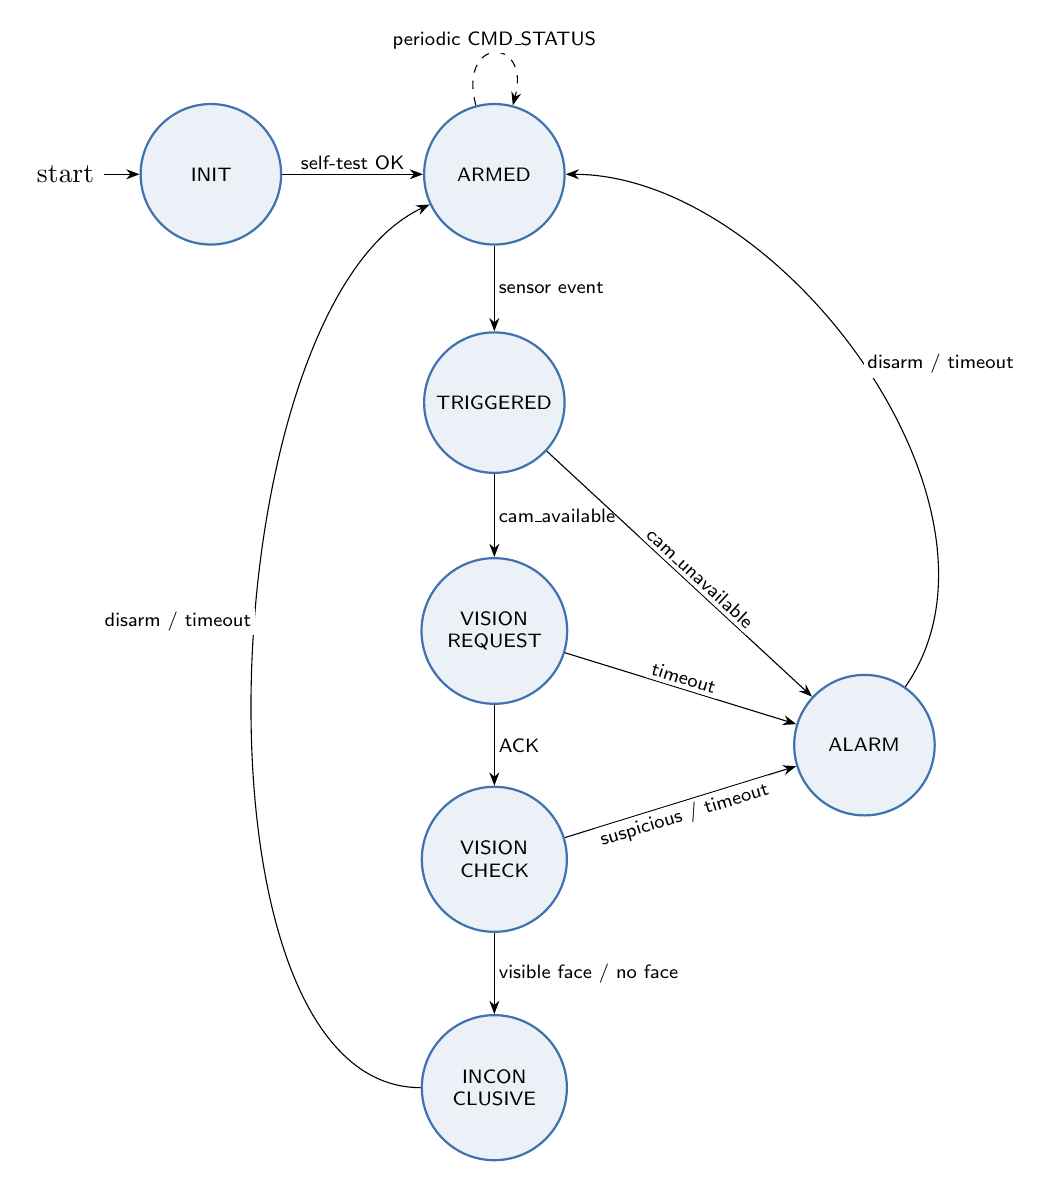
\begin{tikzpicture}[
        every state/.style={
            draw=nodeblue,
            fill=nodeblue!10,
            thick,
            minimum size=1.55cm,
            text width=1.7cm,
            align=center,
            font=\sffamily\scriptsize,
            inner sep=1pt
        },
        >=Stealth,
        lbl/.style={font=\scriptsize\sffamily, fill=white, inner sep=1.4pt}
    ]
        % INIT enters ARMED from the left; the main event pipeline runs downward.
        \node[state, initial] (init) at (-3.6,0) {INIT};
        \node[state] (armed) at (0,0) {ARMED};
        \node[state] (trig)  at (0,-2.9) {TRIGGERED};
        \node[state] (vreq)  at (0,-5.8) {VISION\\REQUEST};
        \node[state] (vchk)  at (0,-8.7) {VISION\\CHECK};
        \node[state] (inc)   at (0,-11.6) {INCON\\CLUSIVE};
        % Single outcome state on the right; all alarm transitions fan into it.
        \node[state] (alarm) at (4.7,-7.25) {ALARM};

        \path[->]
            (init)  edge node[lbl, above] {self-test OK} (armed)
            (armed) edge[loop above, dashed, looseness=5]
                     node[lbl, above] {periodic CMD\_STATUS} (armed)
            (armed) edge node[lbl, right] {sensor event} (trig)
            (trig)  edge node[lbl, right] {cam\_available} (vreq)
            (vreq)  edge node[lbl, right] {ACK} (vchk)
            (vchk)  edge node[lbl, right] {visible face / no face} (inc)
            (trig)  edge node[lbl, above, sloped, pos=0.55] {cam\_unavailable} (alarm)
            (vreq)  edge node[lbl, above, sloped] {timeout} (alarm)
            (vchk)  edge node[lbl, below, sloped] {suspicious / timeout} (alarm)
            (inc)   edge[out=180, in=205, looseness=0.7]
                     node[lbl, left, pos=0.55] {disarm / timeout} (armed)
            (alarm) edge[out=55, in=0, looseness=0.9]
                     node[lbl, right, pos=0.5] {disarm / timeout} (armed);
    \end{tikzpicture}
    \caption{Application Node finite-state machine with camera-availability flag and INCONCLUSIVE state.}
    \label{fig:appnode-fsm}
\end{figure}

\subsection{State behavior table}

\begin{table}[H]
    \centering
    \caption{Application Node state behavior.}
    \label{tab:states}
    \begin{tabular}{@{}l >{\raggedright\arraybackslash}p{9cm}@{}}
        \toprule
        \textbf{State} & \textbf{Behavior} \\
        \midrule
        INIT & Power-on self-test, initialize GPIO/UART, test LED/buzzer, check CAM presence. \\
        ARMED & LED slow blink; sensors active; periodic CAM status query updates \texttt{cam\_available}. \\
        TRIGGERED & Sensor event detected; LED fast blink; branch based on \texttt{cam\_available}. \\
        VISION\_REQUEST & Send CMD\_CAPTURE; wait for ACK with 500~ms timeout and retry logic. \\
        VISION\_CHECK & Maintain fast blink; wait for RSP\_RESULT; enforce 5~s timeout. \\
        INCONCLUSIVE & Non-threat result (visible face / no face); log event; return to ARMED. \\
        ALARM & LED solid, buzzer ON; log event; wait for disarm or timeout. \\
        \bottomrule
    \end{tabular}
\end{table}

% -----------------------------------------------------------------------------
\section{UART protocol interface}
\label{sec:uart}
% -----------------------------------------------------------------------------

The application node is the UART master for the ESP32-CAM module.  Commands and
responses use the binary frame defined in \texttt{docs/firmware/cam\_protocol.md},
which is the authoritative source for the frame layout and the command/response
IDs reproduced here.

\subsection{Frame format}

\begin{center}
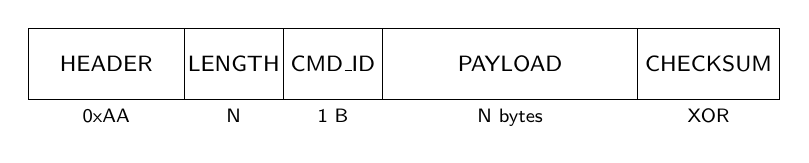
\begin{tikzpicture}[scale=0.9, every node/.style={font=\sffamily\footnotesize}]
    \foreach \x/\w/\txt in {0/2.2/HEADER, 2.2/1.4/LENGTH, 3.6/1.4/CMD\_ID, 5.0/3.6/PAYLOAD, 8.6/2.0/CHECKSUM} {
        \draw (\x,0) rectangle (\x+\w,1) node[midway]{\txt};
    }
    \node[below] at (1.1,0) {\scriptsize 0xAA};
    \node[below] at (2.9,0) {\scriptsize N};
    \node[below] at (4.3,0) {\scriptsize 1 B};
    \node[below] at (6.8,0) {\scriptsize N bytes};
    \node[below] at (9.6,0) {\scriptsize XOR};
\end{tikzpicture}
\end{center}

The checksum is the XOR of all bytes from LENGTH through the end of the payload.

\paragraph{Worked example.}  A \texttt{CMD\_CAPTURE} request (no payload) is the
four bytes \texttt{0xAA 0x01 0x01 0x00}: header \texttt{0xAA}, LENGTH
\texttt{0x01} (CMD\_ID only), CMD\_ID \texttt{0x01}, and checksum
$\texttt{0x01}\oplus\texttt{0x01}=\texttt{0x00}$.  A one-byte \texttt{RSP\_RESULT}
carrying ``suspicious'' (\texttt{0x01}) is \texttt{0xAA 0x02 0x82 0x01 0x81},
where $\texttt{0x02}\oplus\texttt{0x82}\oplus\texttt{0x01}=\texttt{0x81}$.

\subsection{Command set}

\begin{table}[H]
    \centering
    \caption{Application Node command set to the ESP32-CAM.}
    \begin{tabular}{@{}c l >{\raggedright\arraybackslash}p{6.5cm}@{}}
        \toprule
        \textbf{ID} & \textbf{Name} & \textbf{Purpose} \\
        \midrule
        \texttt{0x01} & CMD\_CAPTURE & Request image capture and face-coverage analysis. \\
        \texttt{0x02} & CMD\_STATUS  & Request current module status (updates \texttt{cam\_available}). \\
        \texttt{0x03} & CMD\_RESET   & Request a soft reset of the vision module. \\
        \bottomrule
    \end{tabular}
\end{table}

\subsection{Response handling}

\begin{table}[H]
    \centering
    \caption{Application Node response handling.}
    \begin{tabular}{@{}c l >{\raggedright\arraybackslash}p{6cm}@{}}
        \toprule
        \textbf{ID} & \textbf{Name} & \textbf{Action} \\
        \midrule
        \texttt{0x81} & RSP\_ACK     & Validate echoed command; stop retry timer. \\
        \texttt{0x82} & RSP\_RESULT   & Evaluate result code and drive state transitions. \\
        \texttt{0x83} & RSP\_STATUS   & Update the \texttt{cam\_available} health flag. \\
        \texttt{0x84} & RSP\_ERROR    & Log error; retry command or fall back to basic alarm. \\
        \bottomrule
    \end{tabular}
\end{table}

\subsection{Timeout and retry rules}

\begin{table}[H]
    \centering
    \caption{UART timeout and retry policy.}
    \begin{tabular}{@{}l c l >{\raggedright\arraybackslash}p{4.5cm}@{}}
        \toprule
        \textbf{Operation} & \textbf{Timeout} & \textbf{Retries} & \textbf{Action on failure} \\
        \midrule
        ACK after command & 500~ms & 3 & Mark CAM unresponsive; \texttt{cam\_available=false}; basic alarm. \\
        RESULT after capture & 5~s & --- & Treat as suspicious; activate ALARM. \\
        STATUS response & 500~ms & 2 & \texttt{cam\_available=false} until next successful query. \\
        \bottomrule
    \end{tabular}
\end{table}

\paragraph{Retry loop and the \texttt{disarm} input.}  The retry counts in the
timeout table are applied \emph{inside} the VISION\_REQUEST entry action: the node
re-issues CMD\_CAPTURE up to three times on a missing ACK before the single
``timeout'' transition to ALARM in Figure~\ref{fig:appnode-fsm} fires (the diagram
omits the retry self-loop for clarity).  The \texttt{disarm} event on the return
edges is not a dedicated hardware button --- the board exposes only BOOT/EN --- but
a disarm command received on the USB-CDC / UART0 console, or expiry of the alarm
timeout.

% -----------------------------------------------------------------------------
\section{Firmware design sketch}
\label{sec:sketch}
% -----------------------------------------------------------------------------

The listing below is a design skeleton for the main loop.  It emphasizes state
updates and camera-availability handling rather than production code details.

\begin{lstlisting}[language=C]
void loop() {
    sensors_read(&door_state, &pir_state);

    /* Update camera health flag periodically while armed. */
    if (fsm_state == ARMED && status_query_due()) {
        cam_send_command(CMD_STATUS, NULL, 0);
    }

    fsm_update(door_state, pir_state, cam_result, cam_available);

    if (fsm_state == VISION_REQUEST && !cam_request_pending) {
        cam_send_command(CMD_CAPTURE, NULL, 0);
        cam_request_pending = true;
        timeout_start(CAM_ACK_TIMEOUT_MS);
    }

    cam_process_incoming();   /* parse ACK / RESULT / STATUS / ERROR */
    alarm_update(fsm_state);  /* drive LED and buzzer */
    debug_console_tick();     /* handle USB CLI */
}
\end{lstlisting}

% -----------------------------------------------------------------------------
\section{Additional design considerations}
% -----------------------------------------------------------------------------

\subsection{Mechanical and environmental}

The board is intended for fixed indoor installation near a monitored door.  The
ESP32-CAM mounts on the J3 mezzanine header with its lens facing the entry, so
the enclosure must give the camera a clear field of view and keep the WROOM and
ESP32-CAM PCB antennas over an antenna keep-out (no ground pour) for adequate
Wi-Fi range.  The sensor and USB connectors must remain accessible, and operation
is assumed at normal indoor temperatures; no extended-temperature or outdoor
rating is claimed at this stage.

\subsection{Security considerations}

As a physical-security device the design is intentionally \emph{fail-secure}:
loss of the camera or of CAM communication drives the system to ALARM rather than
silently disarming (\S\ref{sec:statemachine}).  Known, accepted design-stage
limitations are that the USB-CDC / UART0 console is unauthenticated and the
C3$\leftrightarrow$CAM UART link is unencrypted --- acceptable for a wired,
physically protected board, but to be revisited before any networked deployment.
Loss of power and physical tampering remain residual threats; a future revision
could add a tamper input and/or a small backup supply.

% -----------------------------------------------------------------------------
\section{Theoretical verification plan}
% -----------------------------------------------------------------------------

Because no physical prototype is available, verification is limited to
analytical, inspection, and simulation-based activities.

\subsection{Expected behavior and design targets}

\begin{table}[H]
    \centering
    \caption{Design targets for key behaviors.}
    \begin{tabular}{@{}llp{6cm}@{}}
        \toprule
        \textbf{Metric} & \textbf{Target} & \textbf{Rationale} \\
        \midrule
        Sensor-to-alarm latency & $<$ 500~ms & Fast enough to deter an intruder. \\
        ACK timeout & 500~ms & Short enough to detect a stalled CAM. \\
        Capture timeout & 5~s & Allows image capture and inference without excessive delay. \\
        Retry attempts & 3 & Balance robustness against UART noise with responsiveness. \\
        Peak 5~V input current (CAM on) & $\approx$~626~mA & Requires a 5~V/1~A source; bounds F1 and the U4 limit. \\
        Quiescent current (CAM gated off) & $\approx$~90~mA & Monitoring draw stays within a 500~mA USB port. \\
        \bottomrule
    \end{tabular}
\end{table}

\subsection{Analytical verification}

\begin{itemize}
    \item Confirm that every requirement in Table~\ref{tab:requirements} is addressed by at least one design section or artifact.
    \item Walk through the state machine for all combinations of sensor events and \texttt{cam\_available} values to ensure no undefined transitions.
    \item Verify the checksum algorithm for every command and response example in the protocol.
    \item Check the power budget in Table~\ref{tab:power} against the regulator and current-limiter limits.
\end{itemize}

\subsection{Schematic and PCB verification}

\begin{itemize}
    \item Inspect the Altium schematic against the pinout in Table~\ref{tab:pinout}.
    \item Confirm that each GPIO has the correct direction, pull, and protection.
    \item Review the PCB layout against the checklist in \S\ref{sec:electrical}.
    \item Compare the \texttt{assets/Schematic Blocks/} previews with the final schematic before release.
\end{itemize}

\subsection{Excluded verification activities}

The following activities are deferred until a prototype is built:

\begin{itemize}
    \item Oscilloscope capture of sensor and UART signals.
    \item Thermal imaging of the ESP32-C3, ESP32-CAM, and power components.
    \item Measured power consumption under idle, alarm, and capture conditions.
    \item PCB bring-up logs and hardware-in-the-loop tests.
\end{itemize}

% -----------------------------------------------------------------------------
\section{References}
% -----------------------------------------------------------------------------

\begin{enumerate}[label={[\arabic*]}, leftmargin=2.4em]
    \item Espressif Systems, \textit{ESP32-C3-WROOM-02 Datasheet}.
    \item AI-Thinker, \textit{ESP32-CAM Module}; OmniVision, \textit{OV2640 Camera Sensor Datasheet}.
    \item Diodes Incorporated, \textit{AP2112 600\,mA CMOS LDO Datasheet}.
    \item Texas Instruments, \textit{TPS2553 Adjustable Current-Limited Power-Distribution Switch Datasheet}.
    \item Texas Instruments, \textit{SN74LVC2G66 Dual Analog Switch Datasheet}.
    \item STMicroelectronics, \textit{USBLC6-2 Very-Low-Capacitance ESD Protection Datasheet}.
    \item Doeshare, \textit{DN2302S N-Channel MOSFET Datasheet}; TDSEMIC, \textit{SMF5.0CA TVS Datasheet}.
    \item Littelfuse, \textit{1206L Series PTC Resettable Fuse Datasheet}.
    \item Espressif Systems, \textit{ESP-DL} on-device deep-learning library; Google, \textit{TensorFlow Lite for Microcontrollers}.
    \item SecurityNode project artifacts: \texttt{docs/firmware/cam\_protocol.md} (UART protocol), \texttt{docs/application\_node/DESIGN-AUDIT.md} (schematic-vs-docs audit), \texttt{assets/SecurityNode.BomDoc} (bill of materials).
\end{enumerate}

% -----------------------------------------------------------------------------
\section{Summary}
% -----------------------------------------------------------------------------

This application note presented the design of the SecurityNode
controller/application node.  Key design decisions include:

\begin{itemize}
    \item Replacing the unsafe ``CLEAR'' state with an \textbf{INCONCLUSIVE} state for non-threat vision results.
    \item Introducing a \texttt{cam\_available} flag in the ARMED state so the node can gracefully fall back to a basic alarm when the ESP32-CAM is unavailable.
    \item Splitting the event-handling path into TRIGGERED, VISION\_REQUEST, and VISION\_CHECK to separate event detection, command issuance, and result waiting.
    \item Defining requirements, a traceability matrix, and a theoretical verification plan suitable for a design-stage review.
\end{itemize}

The node remains designed to work as a full vision-assisted alarm when the CAM
is present and as a conventional sensor-driven alarm when it is not.  Once
hardware is available, the theoretical plan can be extended with bench
measurements and bring-up results.

\end{document}
